% Шаблон (версия от 15.02.2016) предназначен 
% для использования студентами каф. ПМиИ СамГТУ 
% при оформлении отчетов по лабораторным работам. 
% Для настройки пакета listigs использовался материал 
% статьи Михаила Конника aka virens
% <http://mydebianblog.blogspot.ru/2012/12/latex.html>
% Copyright (c) 2016 by Mikhail Saushkin (msaushkin@gmail.com) 
% All rights reserved except the rights granted by the
% Creative Commons Attribution 4.0 International Licence
% <https://creativecommons.org/licenses/by/4.0/>
% Свежая версия шаблона здесь <https://www.overleaf.com/read/sqvxbnhgxxdm>
\documentclass[14pt,a4paper,report]{ncc}
\usepackage[a4paper, mag=1000, left=2.5cm, right=1cm, top=2cm, bottom=2cm, headsep=0.7cm, footskip=1cm]{geometry}
\usepackage[utf8]{inputenc}
\usepackage[english,russian]{babel}
\usepackage{indentfirst}
\usepackage[dvipsnames]{xcolor}
\usepackage[colorlinks]{hyperref}
\usepackage{listings} 
\usepackage{caption}
\usepackage{amssymb}
\usepackage{tcolorbox}
\DeclareCaptionFont{white}{\color{white}} %% это сделает текст заголовка белым
%% код ниже нарисует серую рамочку вокруг заголовка кода.
\usepackage{color} %% это для отображения цвета в коде
\DeclareCaptionFormat{listing}{\colorbox{gray}{\parbox{\textwidth}{#1#2#3}}}
\captionsetup[lstlisting]{format=listing,labelfont=white,textfont=white}
\lstset{% Собственно настройки вида листинга
inputencoding=utf8, extendedchars=\true, keepspaces = true, % поддержка кириллицы и пробелов в комментариях
language=C++,            % выбор языка для подсветки (здесь это Pascal)
numberstyle =\tiny
basicstyle=\small\sffamily, % размер и начертание шрифта для подсветки кода
keywordstyle =\color{ForestGreen},
numbers=left,               % где поставить нумерацию строк (слева\справа)
numberstyle=\tiny,          % размер шрифта для номеров строк
stepnumber=1,               % размер шага между двумя номерами строк
numbersep=5pt,              % как далеко отстоят номера строк от подсвечиваемого кода
backgroundcolor=\color{white}, % цвет фона подсветки - используем \usepackage{color}
showspaces=false,           % показывать или нет пробелы специальными отступами
showstringspaces=false,     % показывать или нет пробелы в строках
showtabs=false,             % показывать или нет табуляцию в строках
frame=single,               % рисовать рамку вокруг кода
tabsize=2,                  % размер табуляции по умолчанию равен 2 пробелам
captionpos=t,               % позиция заголовка вверху [t] или внизу [b] 
breaklines=true,            % автоматически переносить строки (да\нет)
breakatwhitespace=false,    % переносить строки только если есть пробел
escapeinside={\%*}{*)}      % если нужно добавить комментарии в коде
}

\begin{document}
% Переоформление некоторых стандартных названий
%\renewcommand{\chaptername}{Лабораторная работа}
\def\contentsname{Содержание}

% Оформление титульного листа
\begin{titlepage}
\begin{center}
\textsc{ФГОУ ВО Уральский Федеральный Университет \\ имени первого Президента России Б.Н.Ельцина\\[5mm]
Физико-технологический институт\\[2mm]
Кафедра теоретической физики и прикладной математики}

\vfill

\textbf{ОТЧЁТ ПО ЛАБОРАТОРНОЙ РАБОТЕ №3\\[3mm]
«Моделирование анcамбля частиц при заданной температуре с использованием метода Монте-Карло»\\[6mm]
}
\end{center}

\hfill
\begin{minipage}{.5\textwidth}
Студент:\\[2mm] 
Вялова С.А.\\
группа: ФтМ-170403 \\[5mm]

Преподаватель:\\[2mm] 
д.ф.-м.н., профессор\\
Мазуренко Владимир Владимирович\\[5mm]

Консультант:\\[2mm] 
н.с.\\
Сотников Олег Михайлович\\

\end{minipage}%
\vfill
\begin{center}
\today  \\
%\theyear\, г.
 Екатеринбург.
\end{center}
\end{titlepage}

% Содержание
\tableofcontents
\newpage
\chapter{Моделирование анcамбля частиц при заданной температуре с использованием метода Монте-Карло}
\section{Цель работы}


Разработка программы для моделирования основного состояния двумерных решеток, в которых частицы взаимодействуют через потенциал Леннарда-Джонса методом Монте-Карло (алгоритм Метрополиса).
\

В ходе выполнения работы необходимо реализовать следующие пункты:
\begin{itemize}
\item Реализовать расчёт погрешности полной энергии;
\item провести сравнение с результатами молекулярной динамики, полученны-
ми в предыдущих заданиях через решение уравнений движения.;

\end{itemize}

\

\newpage\section{Теоретическая часть }
\subsection{Потенциал Леннарда-Джонса}
%text
Потенциал Леннарда-Джонса представляет собой простую модель парного взаимодействия неполярных молекул, описывающая зависимость энергии взаимодействия двух частиц от расстояния между ними.
Потенциал был предложен Леннардом-Джонсом первоначально для исследования термодинамических свойств инертных газов. Наиболее часто используется так называемый (6-12)-потенциал Леннарда-Джонса, записанный в форме 
\
\begin{equation}
 U = 4 \cdot \varepsilon \cdot [(\sigma/r)^{12} - (\sigma/r)^{6}  ] ,
 \end{equation} 
где $\varepsilon$ - глубина потенциальной ямы, $\sigma$ - значение расстояния между частицами, при котором потенциал равен нулю. Шестая степень убывания отвечает электростатическому диполь-дипольному и дисперсионному притяжению; двенадцатая степень убывания потенциала моделирует достаточно жесткое отталкивание и выбрана из соображений математического удобства.
\

\subsection{Метод Монте Карло}
Методы Монте Карло —-- численные методы решения задач при помощи моделирования случайных величин и статистической оценки их характеристик. Они нашли применение в самых разнообразных областях, таких как вычисление интегралов и решение интегральных уравнений, решение дифференциальных уравнений в частных производных, систем алгебраических уравнений, моделирование различных фазовых переходов, решение задач перколяционной теории, описание моделей статистической физики и даже жизненных циклов простейших организмов. Хотя методы Монте Карло и основаны на использовании случайных величин, решаемая задача не обязательно должна иметь вероятностный характер.

Плюсы использования стохастических методов состоят в том, что многие математические и физические задачи либо не имеют известных аналитических методов решения, либо их реализация требует значительных вычислительных затрат. Применение случайных величин позволяет значительно ускорить и упростить решение таких задач. Еще одно преимущество данного подхода заключается в том, что таким образом можно провести имитацию реального физического эксперимента.

Для физических задач, в ходе моделирования эксперимента происходит накопление статистических данных. Наблюдаемые величины в таком случае строятся как среднее значение от большого числа вычислений. 

К примеру, вероятность некоего процесса задается распределением Гиббса:

\begin{equation}
P=\frac{1}{Z}e^{-\frac{H}{kT}},  
\end{equation}
где $k$ --- коэффициент Больцмана, $T$ --- температура, $Z$ --- нормировочная константа (статистическая сумма). 

При постановке такой задачи в статистической физике среднее значение некоторой величины считалось бы по формуле следующего типа:
\begin{equation}
\left\langle A(x)\right\rangle=\frac{\sum_{i=1}^NA(x_i)e^{-\frac{H(x_i)}{kT}}}{\sum_{i=1}^Ne^{-\frac{H(x_i)}{kT}}},
\end{equation}
где $A(x_i)$  --- значение величины, измеренное в точке $x_i$ фазового пространства.

Расчеты по этой формуле достаточно громоздки и занимают значительное время, к тому же перебор всех существующих конфигураций большой системы является невозможным.

Однако, при большом числе опытов в состояниях, близких к равновесному, это выражение можно заменить на:

\begin{equation}
\left\langle A(x)\right\rangle=\frac{\sum_{i=1}^{N_{MC}}A(x_i)}{N_{MC}},
\end{equation}

Таким образом, расчеты с использованием метода Монте Карло сводятся к вычислению арифметического среднего значения, что значительно ускоряет процесс.

\subsection{Алгоритм Метрополиса}
Таким образом, у нас есть двумерная система частиц, которые могут смещаться случайным образом в пределах некой окружности вблизи начального положения, но так, что можно достичь состояния с любой энергией за конечное количество шагов (условие эргодичности). Для конечных температур следует ожидать, что энергия системы должна флуктуировать вокруг некоторого равновесного значения. Чтобы вычислять термодинамические величины необходимо разыгрывать состояния таким образом, чтобы система пришла к состоянию равновесия за какое-то разумное время. Для этих целей и служит Алгоритм Метрополиса. Его можно разбить на следующие шаги:

\vspace{8mm}
\begin{enumerate}
\item сгенерировать начальную конфигурацию системы $\alpha_k$;
\item выбрать $i$-ую частицу и сместить ее, сгенерировав тем самым пробное состояние системы  $\alpha_i$;
\item вычислить энергию нового состояния $E_i$;
\item если $E_k>E_i$, принять новое состояние системы;
\item если $E_i>E_k$, принять новое состояние с вероятностью:\\
$R=exp(\Delta E/kT)$;
\begin{itemize}
\item выбрать случайное число $0\le r\le 1$
\item положить состояние 
\[
\alpha_{k+1}=
\begin{cases}
\alpha_k, & \text{если $R\ge r$;} \\
\alpha_i, & \text{если $R<r$.}
\end{cases}
\]
\end{itemize}
\item вычислить нужные величины в состоянии $\alpha_{k+1}$, взять его за начальное и повторять с пункта 2 нужное количество шагов.
\end{enumerate}

\newpage
\subsection{Описание  методов}
%text
В ходе работы необходимо реализовать квазидинамику систему, используя алгоритм Метрополиса. Для этого необходимо задать начальные положения атомов ${r^{N=0}}$, в которой $N$ - номер шага алгоритма Метрополиса, сместить $i$-ю частицу на малое произвольное число , выбранное в промежутке  ${-\delta, -\delta]$, вычислить энергию системы со смещенной $i$-й частицей, и, в зависимости от того, является ли разность энергии предыдущей конфигурации и полученной положительной или отрицательной, сохранить систему в таком состоянии либо вернуть в предыдущее состояние. Данная операция повторяется для всех остальных частиц, и число таких операций определяется параметром $N$.

\

Энергия решетки вычисляется через потенциал Леннарда-Джонса следующим образом:
\begin{equation}
E=4 \varepsilon \sum\limits_{i=1}^N \sum\limits_{s=i+1}^N{ [(\sigma/\vec{r}_{is})^{12} - (\sigma/\vec{r}_{is})^{6}  ]}
\end{equation}
\

Характерный вид начального расположения атомов в треугольной и квадратной решетках  $L_x=7$ представлен на рисунках \ref{ris:image1} и \ref{ris:image2}. 

\begin{figure}[h]
\center{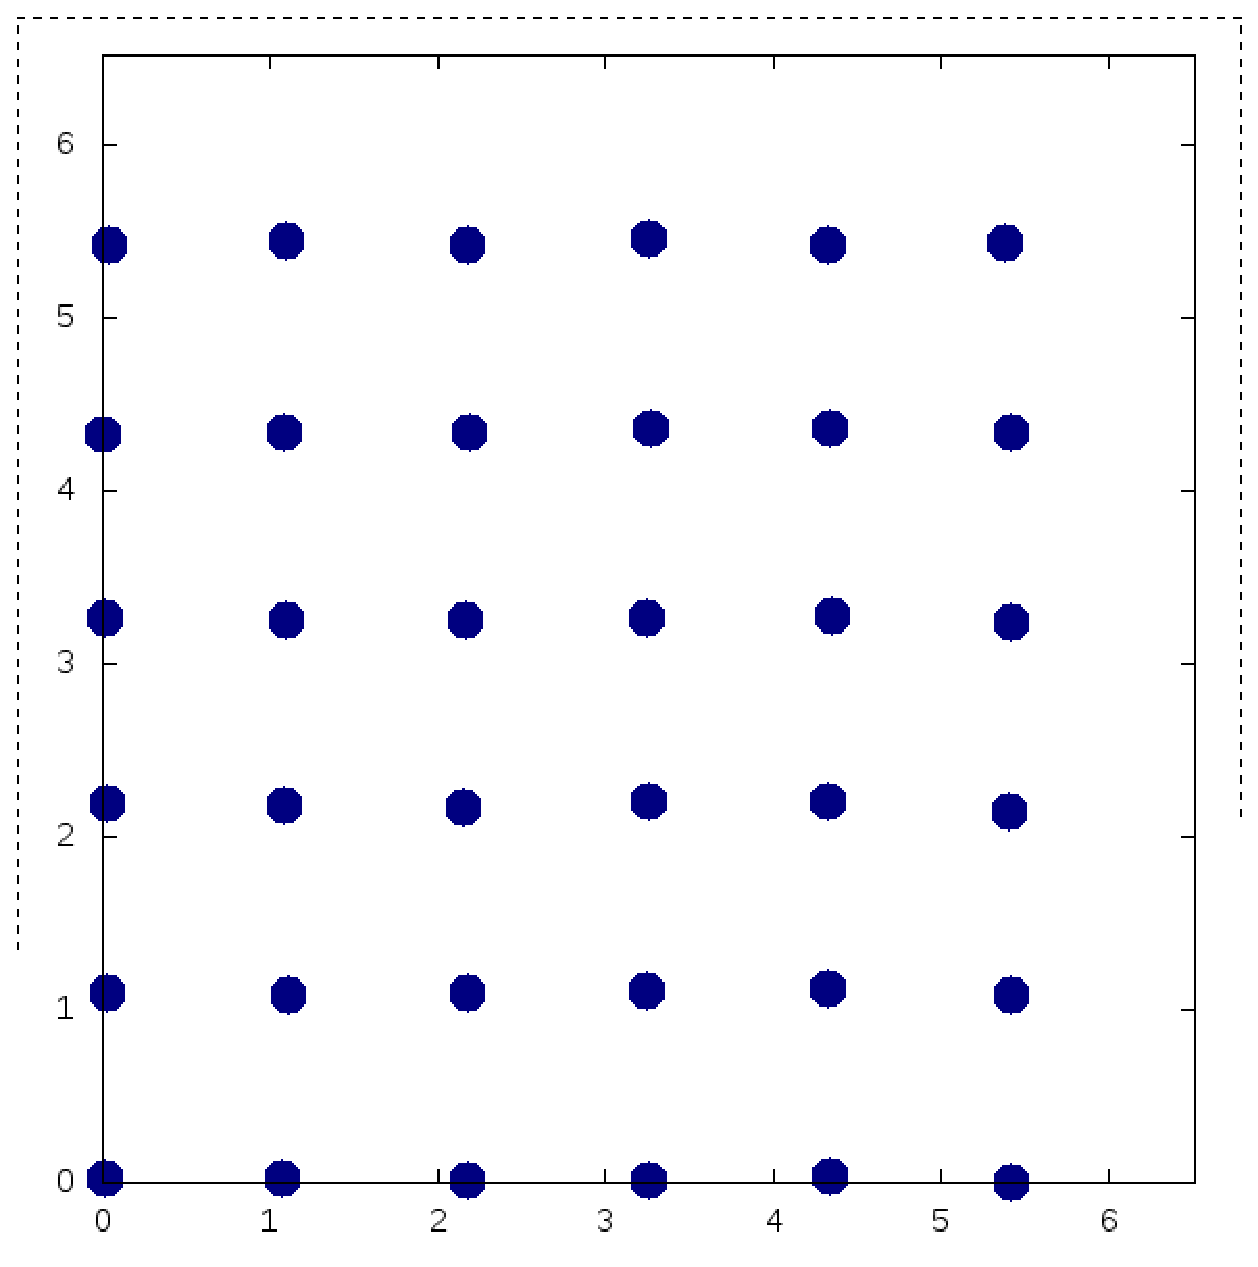
\includegraphics[width=0.6\linewidth]{pictures/system_initial_sq}}
\caption{Расположение атомов в квадратной решетке.}
\label{ris:image1}
\end{figure}
\

\begin{figure}[h]
\center{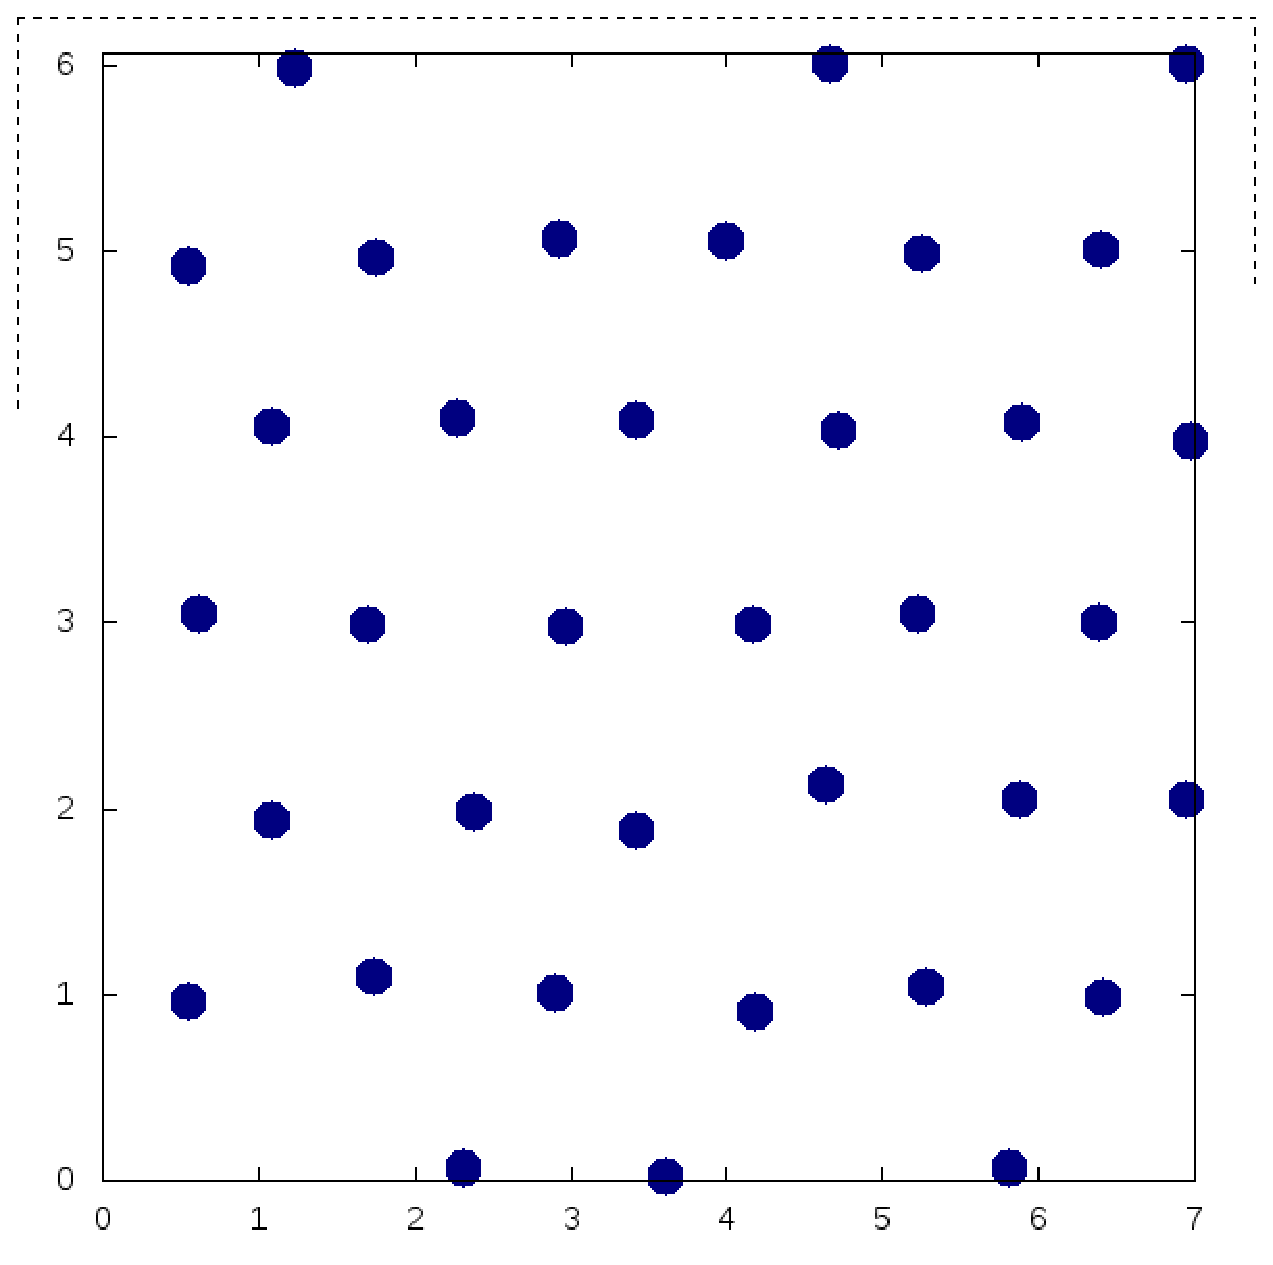
\includegraphics[width=0.6\linewidth]{pictures/system_initial}}
\caption{Расположение атомов в треугольной решетке.}
\label{ris:image2}
\end{figure}
\
\subsection{Разработка программной части}
Для решения поставленной задачи была разработана программа на языке С++. Задача программы - реализовать квазидинамику двумерной системы частиц, взаимодействующих через потенциал Леннарда-Джонса, при использовании алгоритма Метрополиса.
\

В программе имеется возможность задать тип решетки - треугольную либо квадратную, линейные размеры системы, число частиц в системе, параметры потенциала - $\sigma$ и $\epsilon$, пределы смещения частиц $\delta$, значения температурного множителя $kT$, число шагов алгоритма Метрополиса $N$, а также частоту записи значений энергии системы, среднеквадратического смещения в файлы.
\
Программа выводит в файлы значения энергии системы от шага алгоритма Метрополиса, значение среднеквадратического смещения частиц системы в зависимости от шага алгоритма, траекторию одной из частиц. 
Значения энергии на каждом шаге, среднеквадратического смещения на каждом шаге, а также номер шага моделирования выводятся в терминал. 

\ 

При исследовании системы были использованы следующие входные данные:
\begin{itemize}
\begin{itemize}
\item максимальное смещение координаты $\delta=0.005$;
\item $\sigma^{L_{x}=7}_{n=36}=0.985$ для квадратной решетки;
\item $\sigma^{L_{x}=7}_{n=36}=1.047$ для треугольной решетки;
\item температурный множитель $kT=0.0000001$, $kT=0.01$
\end{itemize}
\item линейный размер системы по горизонтали ${L_x=7}$ для треугольной решетки;
\item линейный размер системы по горизонтали ${L=L_x\sqrt{\sqrt{3}/2}}$ для квадратной решетки, где  ${L_x=7}$ ;
\item число частиц в решетке ${n=36}$;
\item число шагов алгоритма Метрополиса ${N=30000}$;
\end{itemize}

Программа запускается из командной оболочки bash. Снимок экрана с выводом программы представлен на рисунке \ref{ris:image3}.
\

\begin{figure}[h]
\center{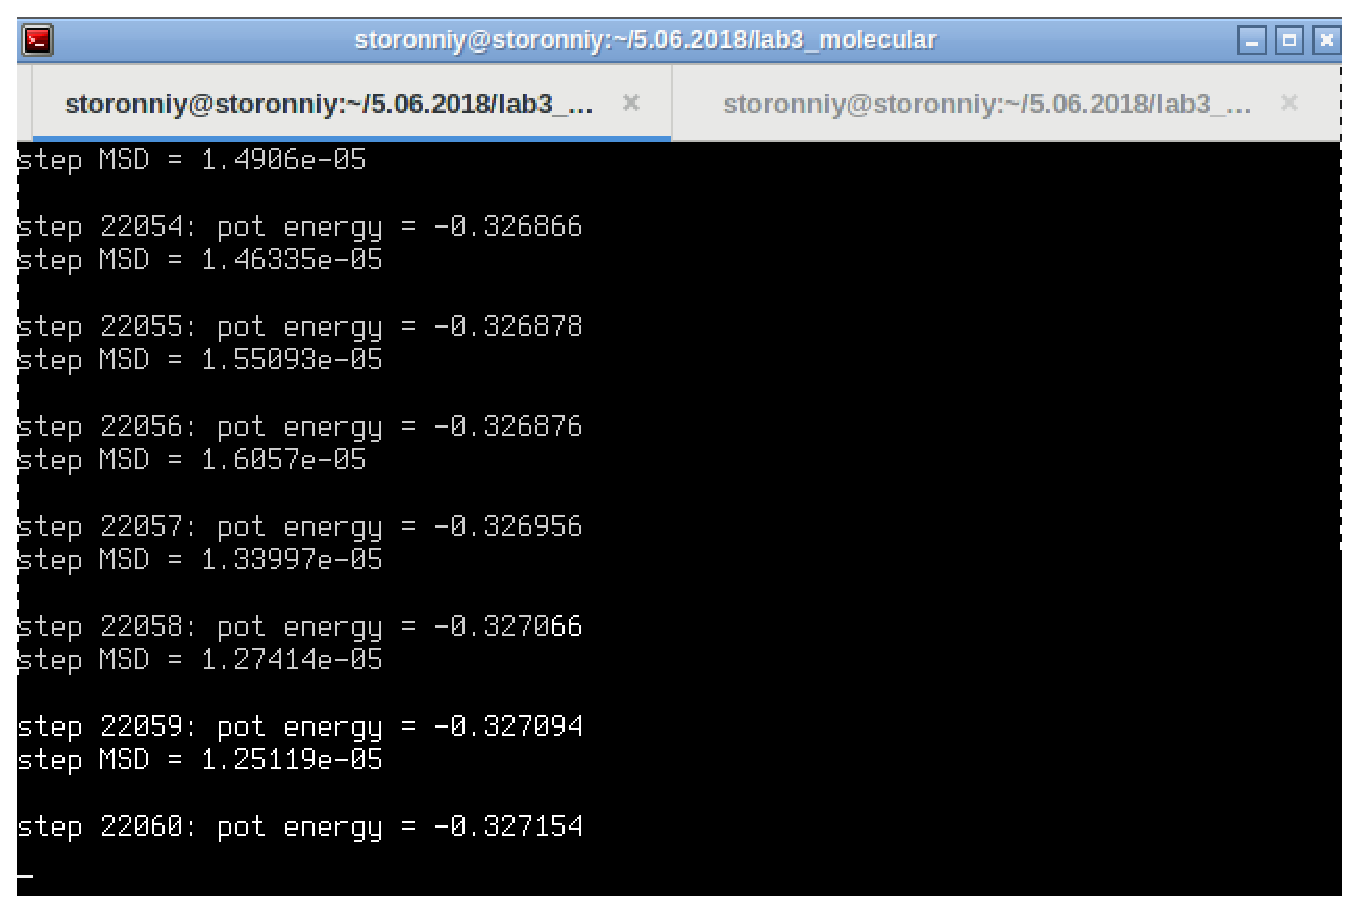
\includegraphics[width=1\linewidth]{pictures/program}}
\caption{Демонстрация выполняющейся программы.}
\label{ris:image3}
\end{figure}
\


 \subsection{Результаты моделирования}
Для начала рассмотрим систему, начальное положение которой задаётся как на рисунке \ref{ris:image1} - то есть квадратную решетку.
\

 В результате моделирования, были получены графики зависимости энергии системы (\ref{ris:image4})  для каждого значения шага алгоритма $N$, среднеквадратического смещения (\ref{ris:image5}), а также траектория одной из частиц системы (\ref{ris:image6}). Характерный вид системы после нескольких шагов квазидинамики для квадратной решетке представлен на рисунке \ref{ris:image7}


 \
 \begin{figure}[h!]
\center{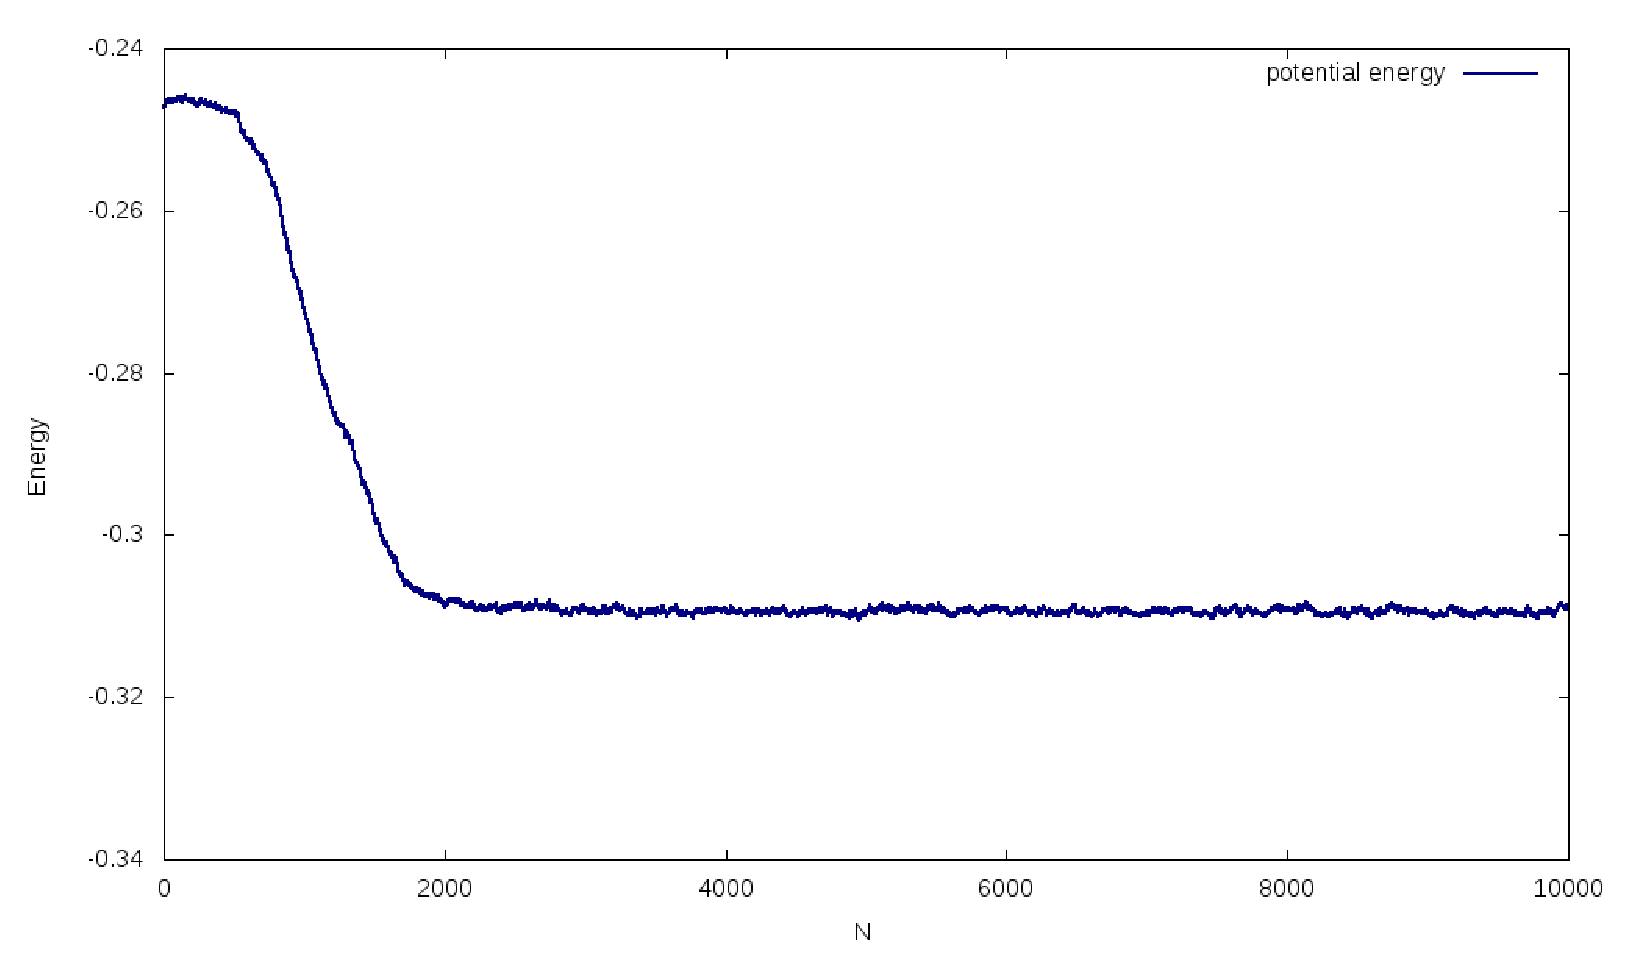
\includegraphics[width=0.6\linewidth]{pictures/energy_sq}}
\caption{График зависимости энергии системы в зависимости от номера шага алгоритма Метрополиса для квадратной решетки.}
\label{ris:image4}
\end{figure}
  \begin{figure}[h!]
\center{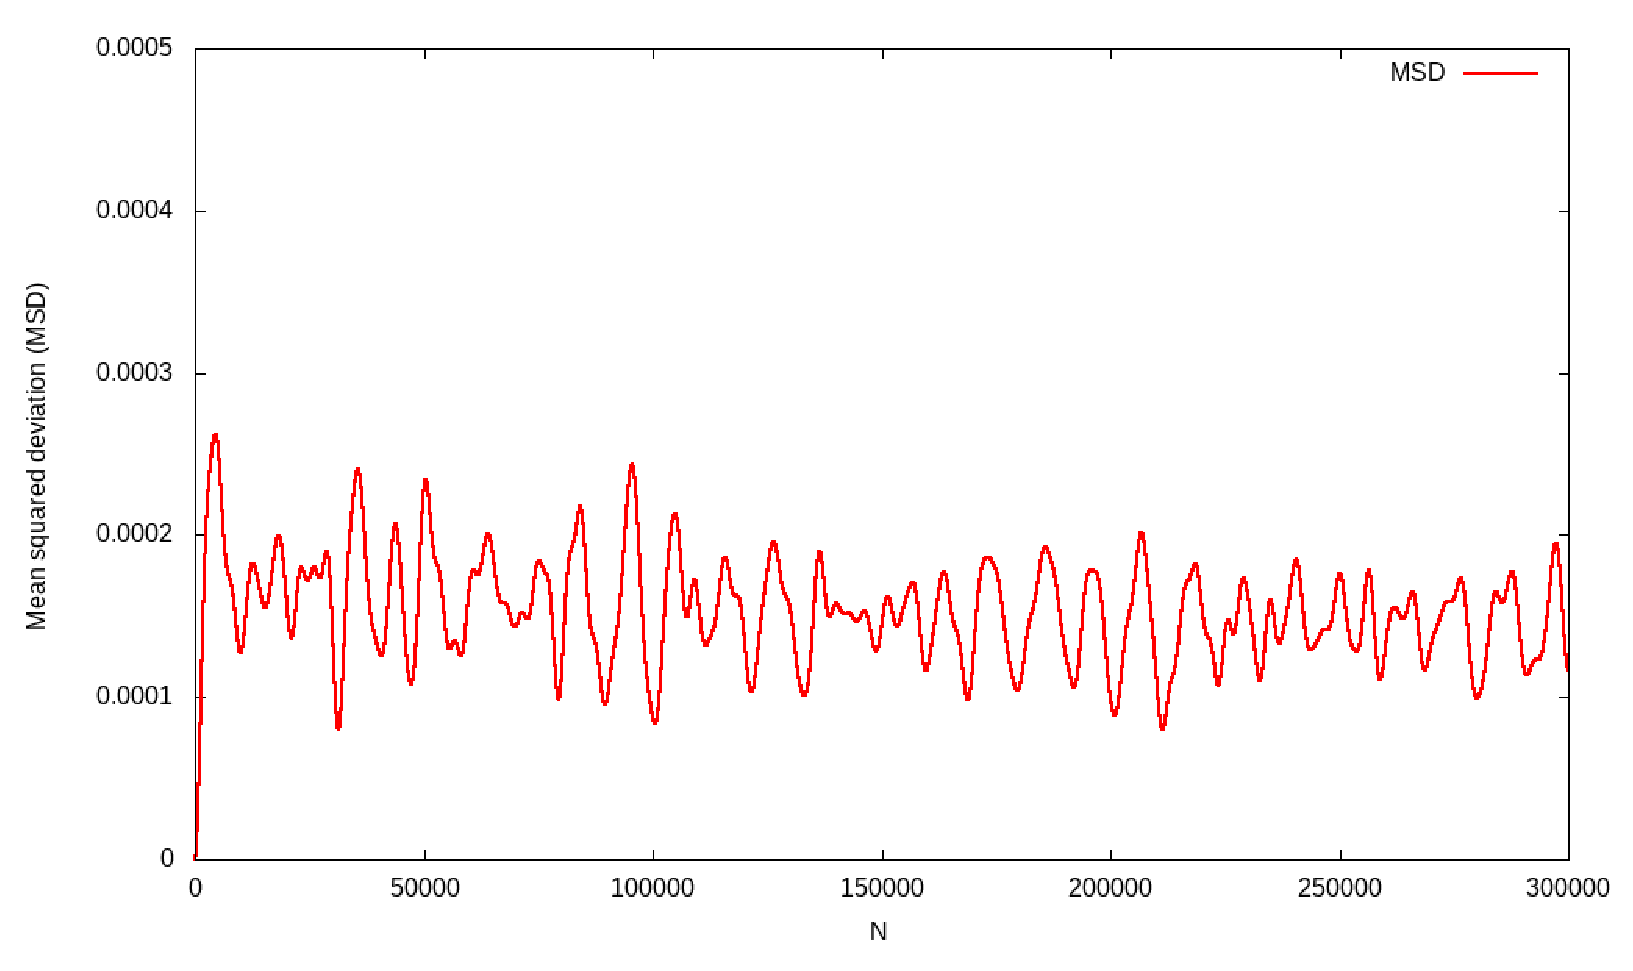
\includegraphics[width=0.6\linewidth]{pictures/MSDsq}}
\caption{График зависимости среднеквадратического смещения от номера шага алгоритма Метрополиса}
\label{ris:image5}
\end{figure}
  \begin{figure}[h!]
\center{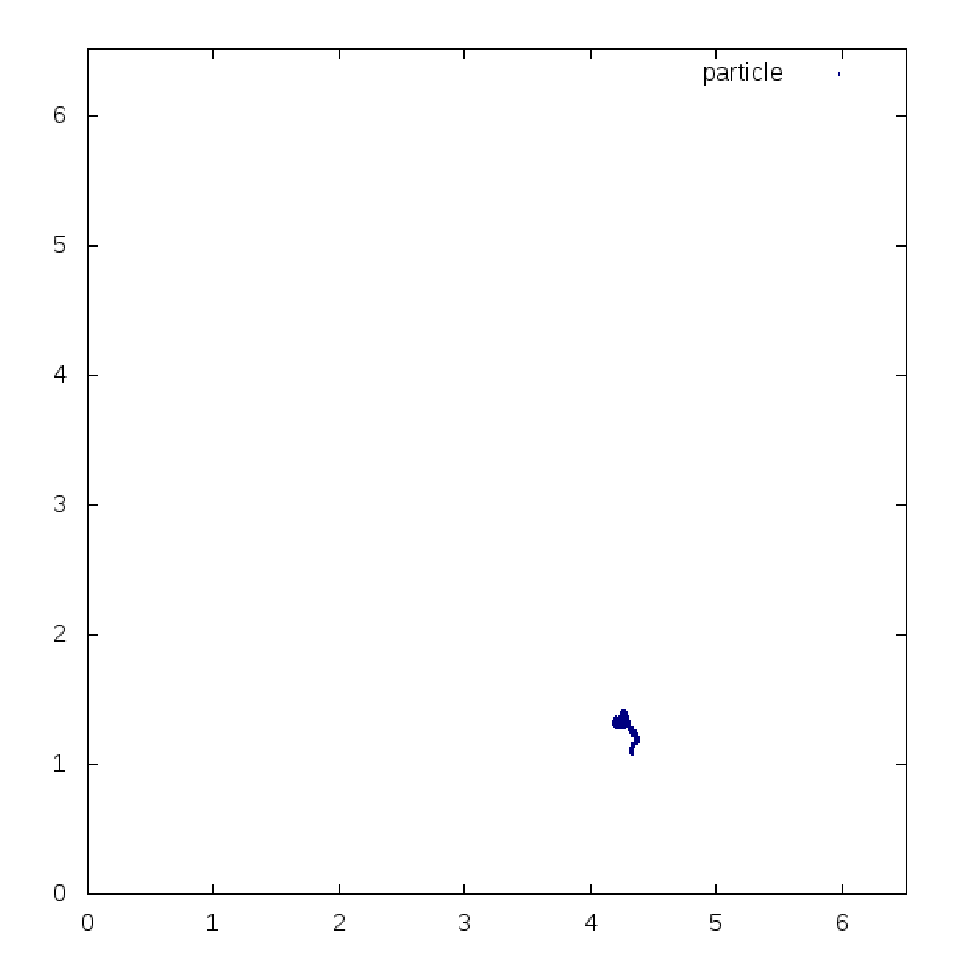
\includegraphics[width=0.6\linewidth]{pictures/particle_sq}}
\caption{Траектория одной из частиц}
\label{ris:image6}
\end{figure}
  \begin{figure}[h!]
\center{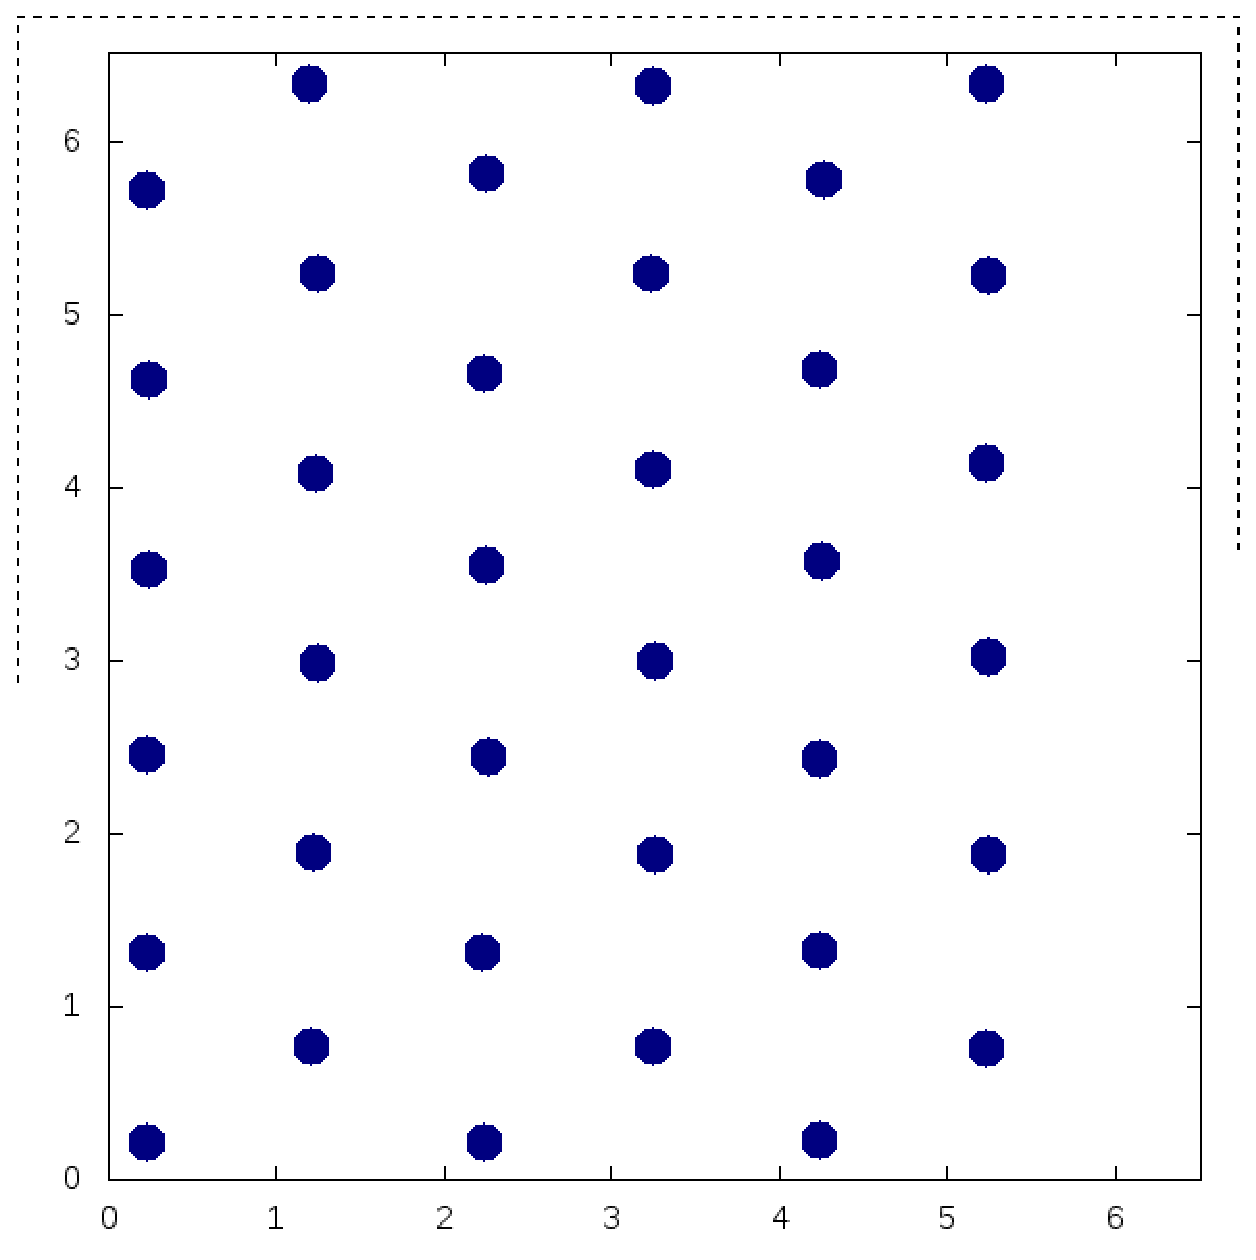
\includegraphics[width=0.6\linewidth]{pictures/system_sq}}
\caption{Состояние системы после некоторого числа шагов моделирования}
\label{ris:image7}
\end{figure}
\


Из полученной квазидинамики видно, что после некоторого числа шагов моделирования система приходит к некоторому равновесному состоянию с меньшей энергией, в котором стремится стабилизироваться, даже при очень малом значении температурного множителя $kT=0,0000001$. Система переходит из квадратного упорядочения к треугольному, энергия системы понижается до некоторого равновесного, как видно из графика энергии системы, представленного на рисунке \ref{ris:image4}.


\
Далее была рассмотрена система с другим начальным упорядочением частиц, характерный вид которого представлен на рисунке \ref{ris:image2}. Энергия данной системы в ходе моделирования изменялась, как показано на рисунке \ref{ris:image8}, что говорит о том, что данная конфигурация решетки является стабильной, и энергия такой системы балансирует у равновесного значения.
\
Состояние такой системы после некоторого количества шагов моделирования представлено на рисуке \ref{ris:image9}. График среднеквадратического смещения для данного случая представлен на рисунке \ref{ris:image10}, из которого ясно, что смещения частиц крайне малы - система стабильна в исходном положении.
\
 \begin{figure}[h!]
\center{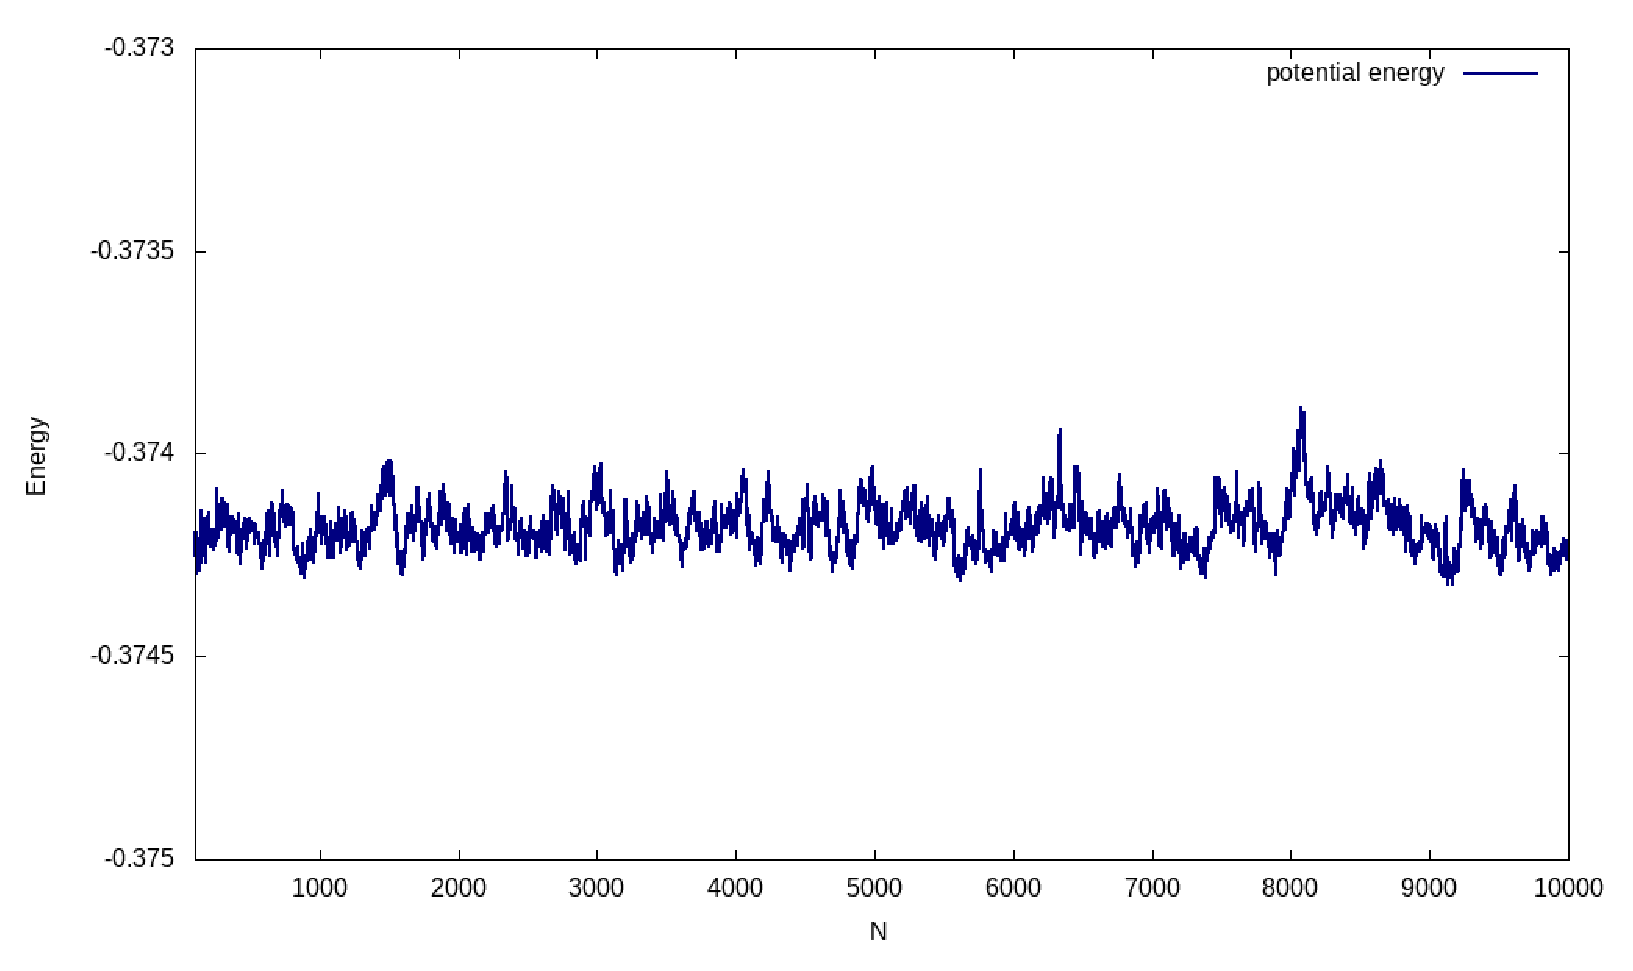
\includegraphics[width=0.6\linewidth]{pictures/energy_tr}}
\caption{График зависимости энергии системы в зависимости от номера шага алгоритма Метрополиса для треугольной решетки.}
\label{ris:image8}
\end{figure}
\

  \begin{figure}[h!]
\center{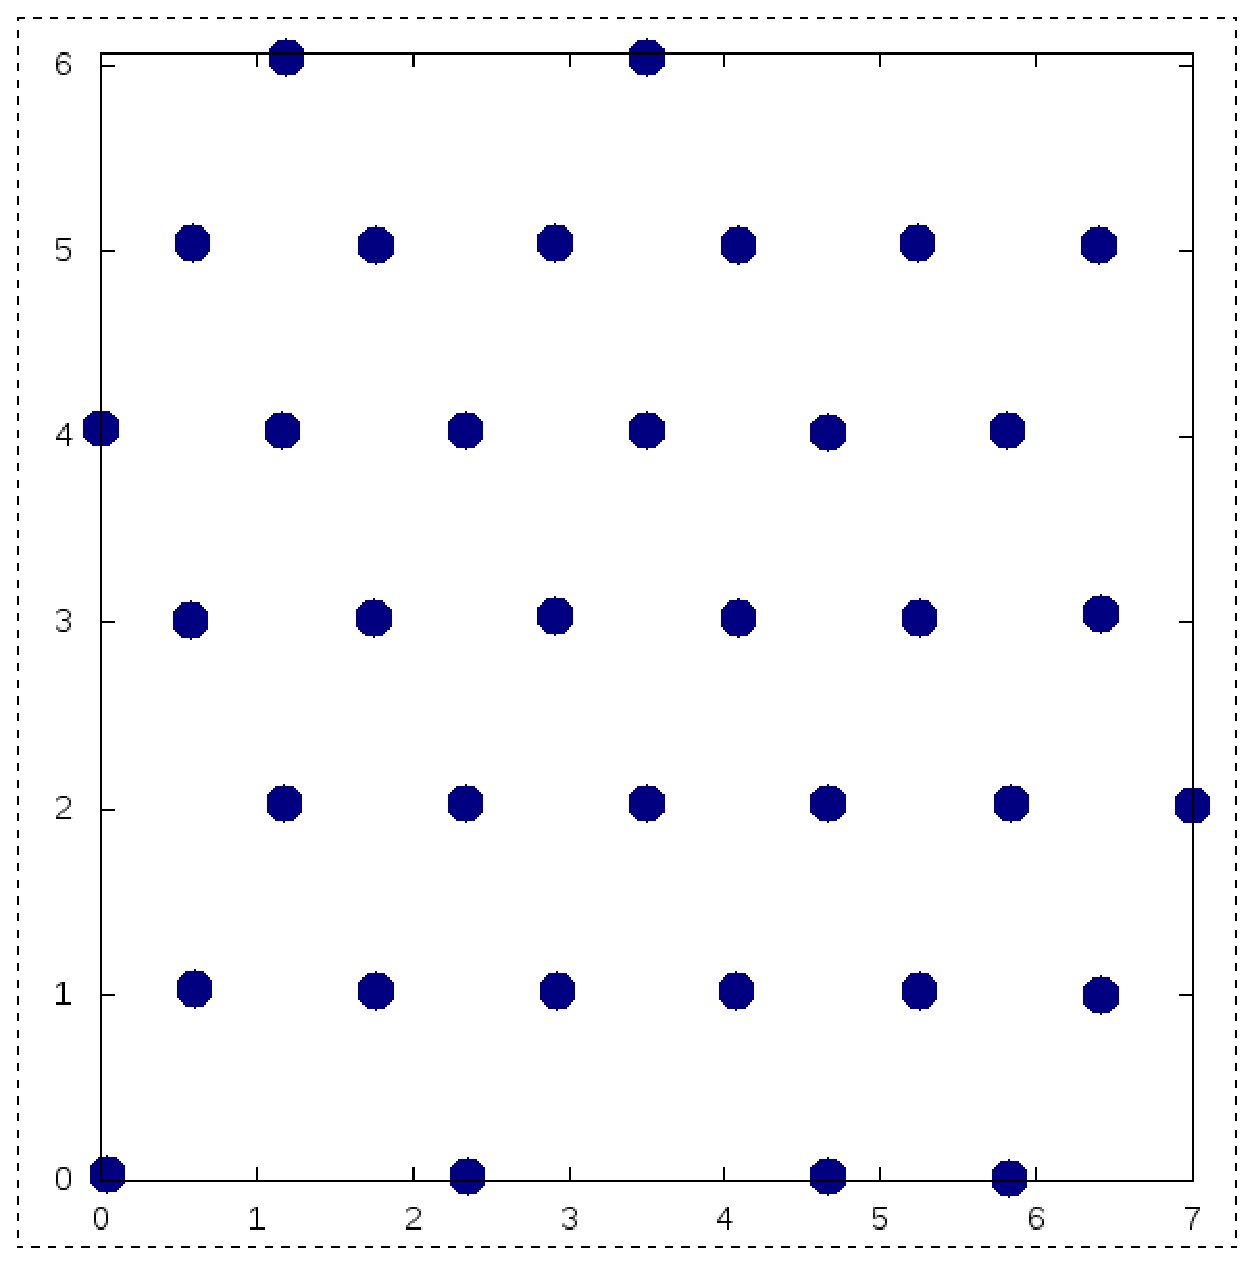
\includegraphics[width=0.6\linewidth]{pictures/system_triangle}}
\caption{Состояние системы после некоторого числа шагов моделирования}
\label{ris:image9}
\end{figure}
\

  \begin{figure}[h!]
\center{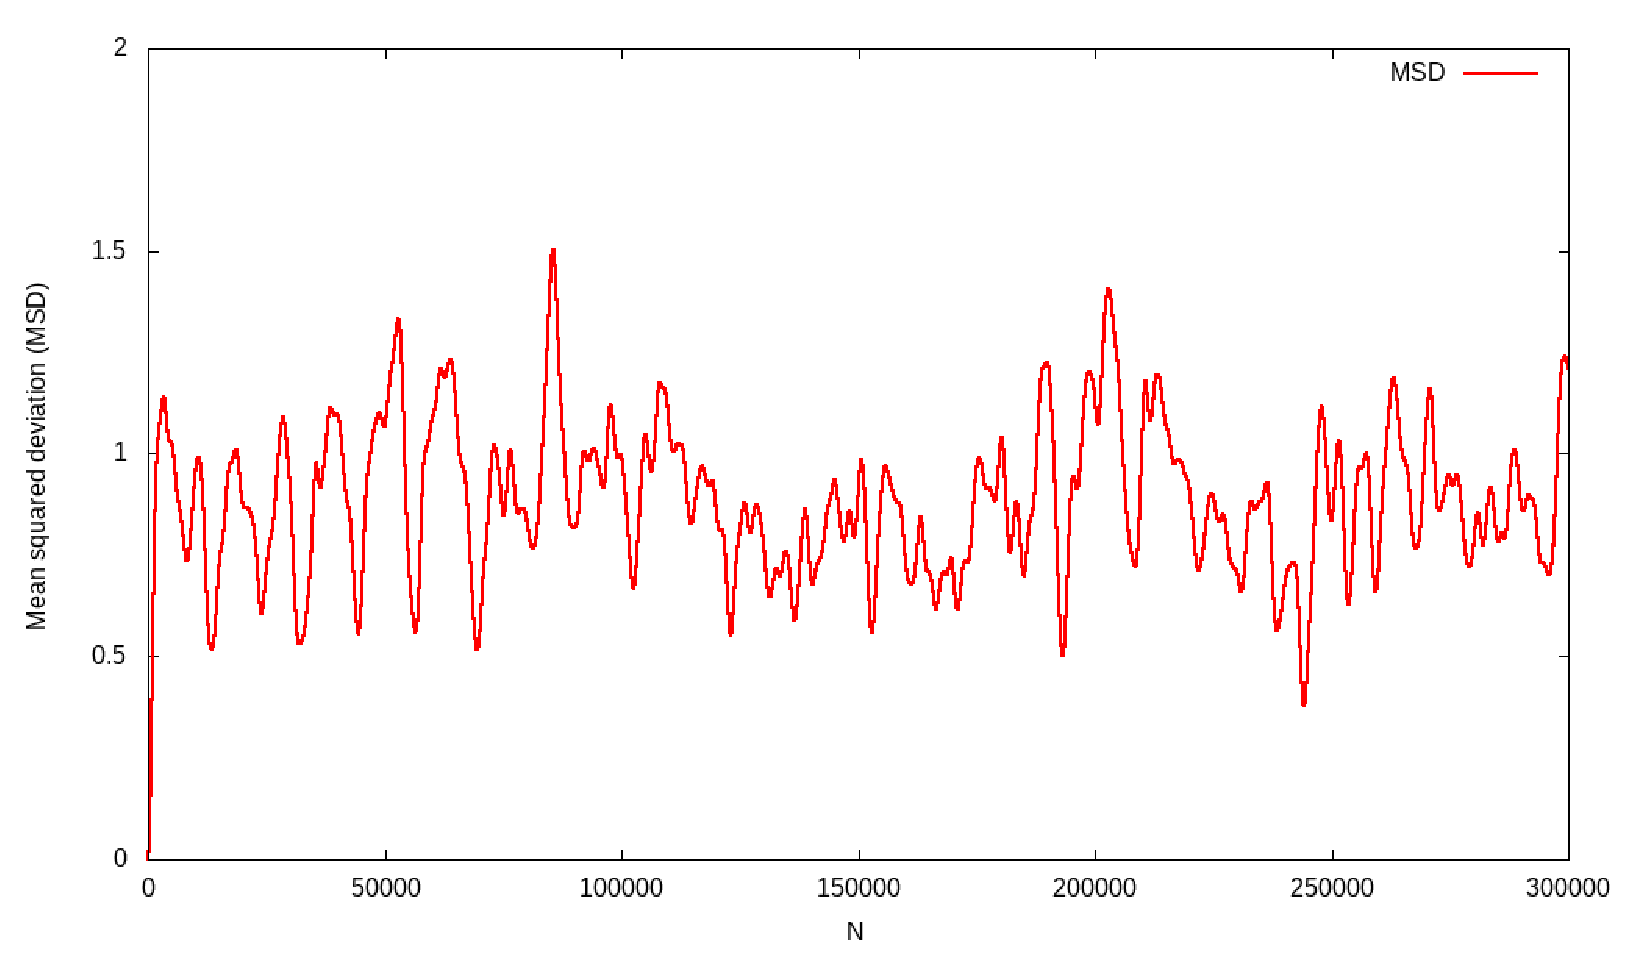
\includegraphics[width=0.6\linewidth]{pictures/MSD_tr}}
\caption{График зависимости среднеквадратического смещения от номера шага алгоритма Метрополиса}
\label{ris:image10}
\end{figure}

Попробуем "разрушить" треугольную решетку, увеличив температурный множитель до $kT=0,01$. В результате моделирования данной ситуации, получаем график зависимости энергии системы в ходе квазидинамики, представленный на рисунке \ref{ris:image11}, из которого легко видеть, что энергия системы на первых шагах алгоритма растёт вверх от основного состояния для данного числа частиц, линейных размеров системы и параметра $\sigma$. Это означает, что частицы смещаются из узлов треугольной решетки, тем самым разрушая её. Данное предположение подтверждается траекторией движения отдельной частицы, представленной на рисунке \ref{ris:image12}, которая сигнализирует о значительном смещении отдельной частицы системы из начального положения, чего не наблюдалось в случае более малого значения температурного множителя $kT$. Характерный вид системы после некоторого числа шагов моделирования представлено на рисунке \ref{ris:image13}, который указывает на разрушение решетки. График зависимости среднеквадратического смещения представлен на рисунке \ref{ris:image14}.
\
 \begin{figure}[h!]
\center{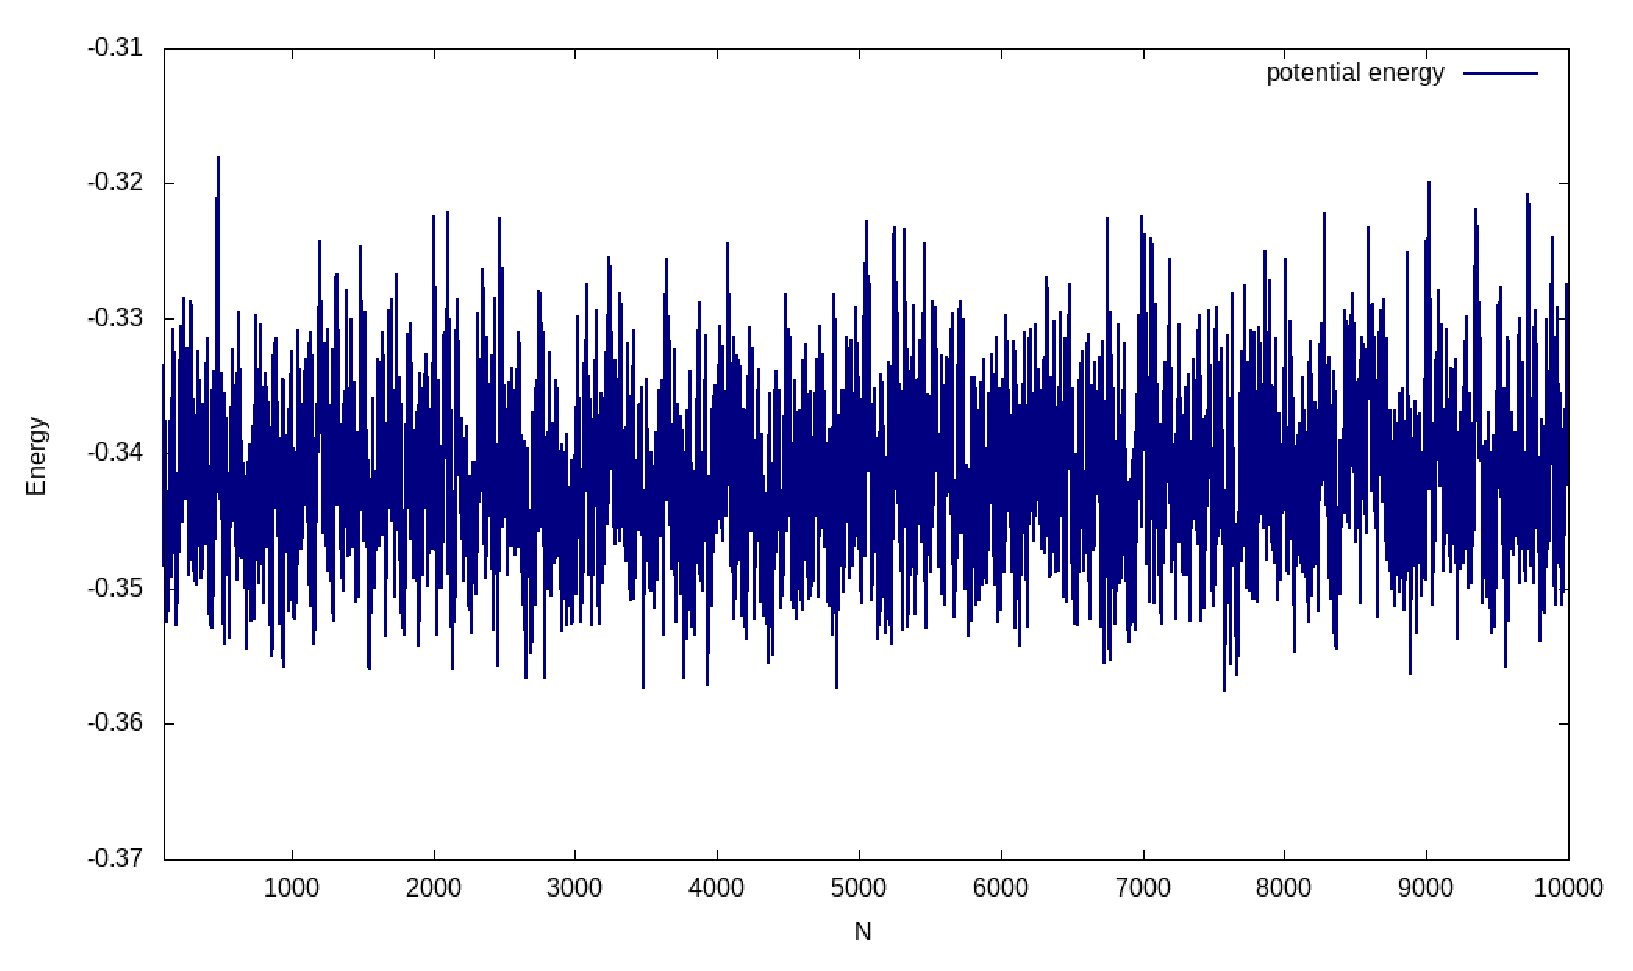
\includegraphics[width=0.6\linewidth]{pictures/energy_crash}}
\caption{График зависимости энергии системы в зависимости от номера шага алгоритма Метрополиса для треугольной решетки.}
\label{ris:image11}
\end{figure}
  \begin{figure}[h!]
\center{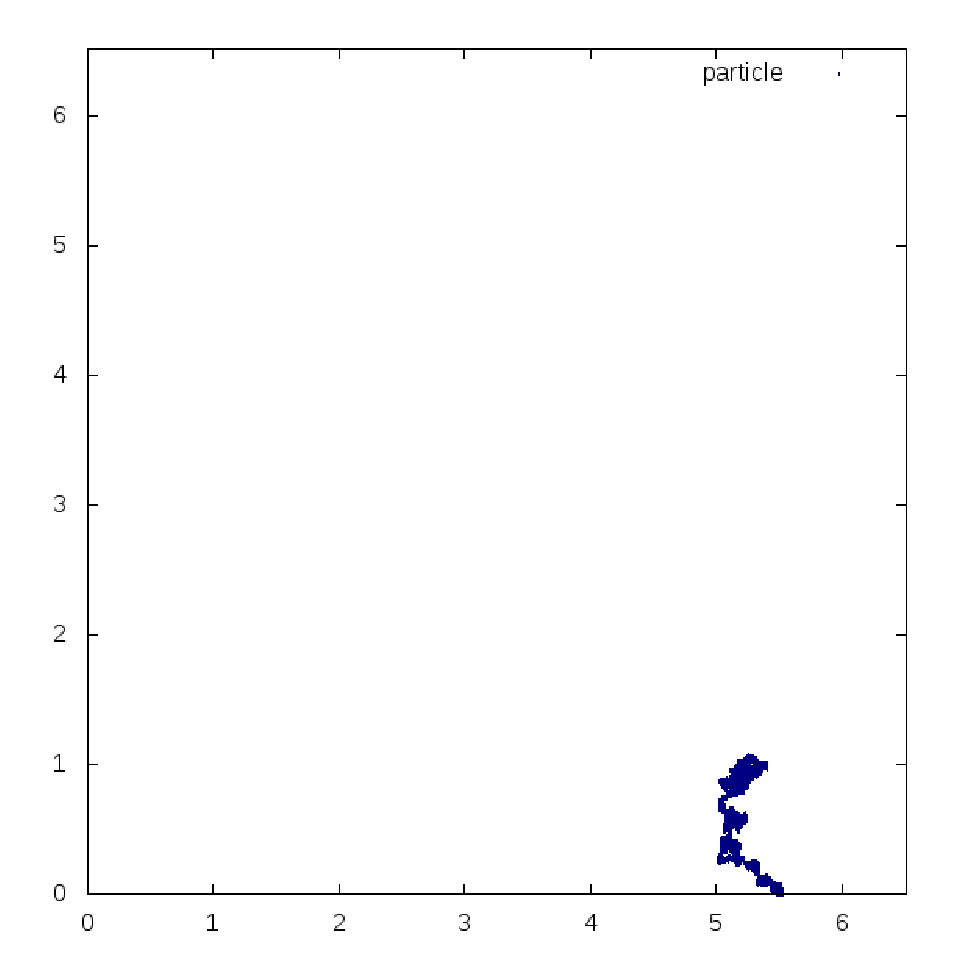
\includegraphics[width=0.6\linewidth]{pictures/particle_crash}}
\caption{Траектория одной из частиц}
\label{ris:image12}
\end{figure}
  \begin{figure}[h!]
\center{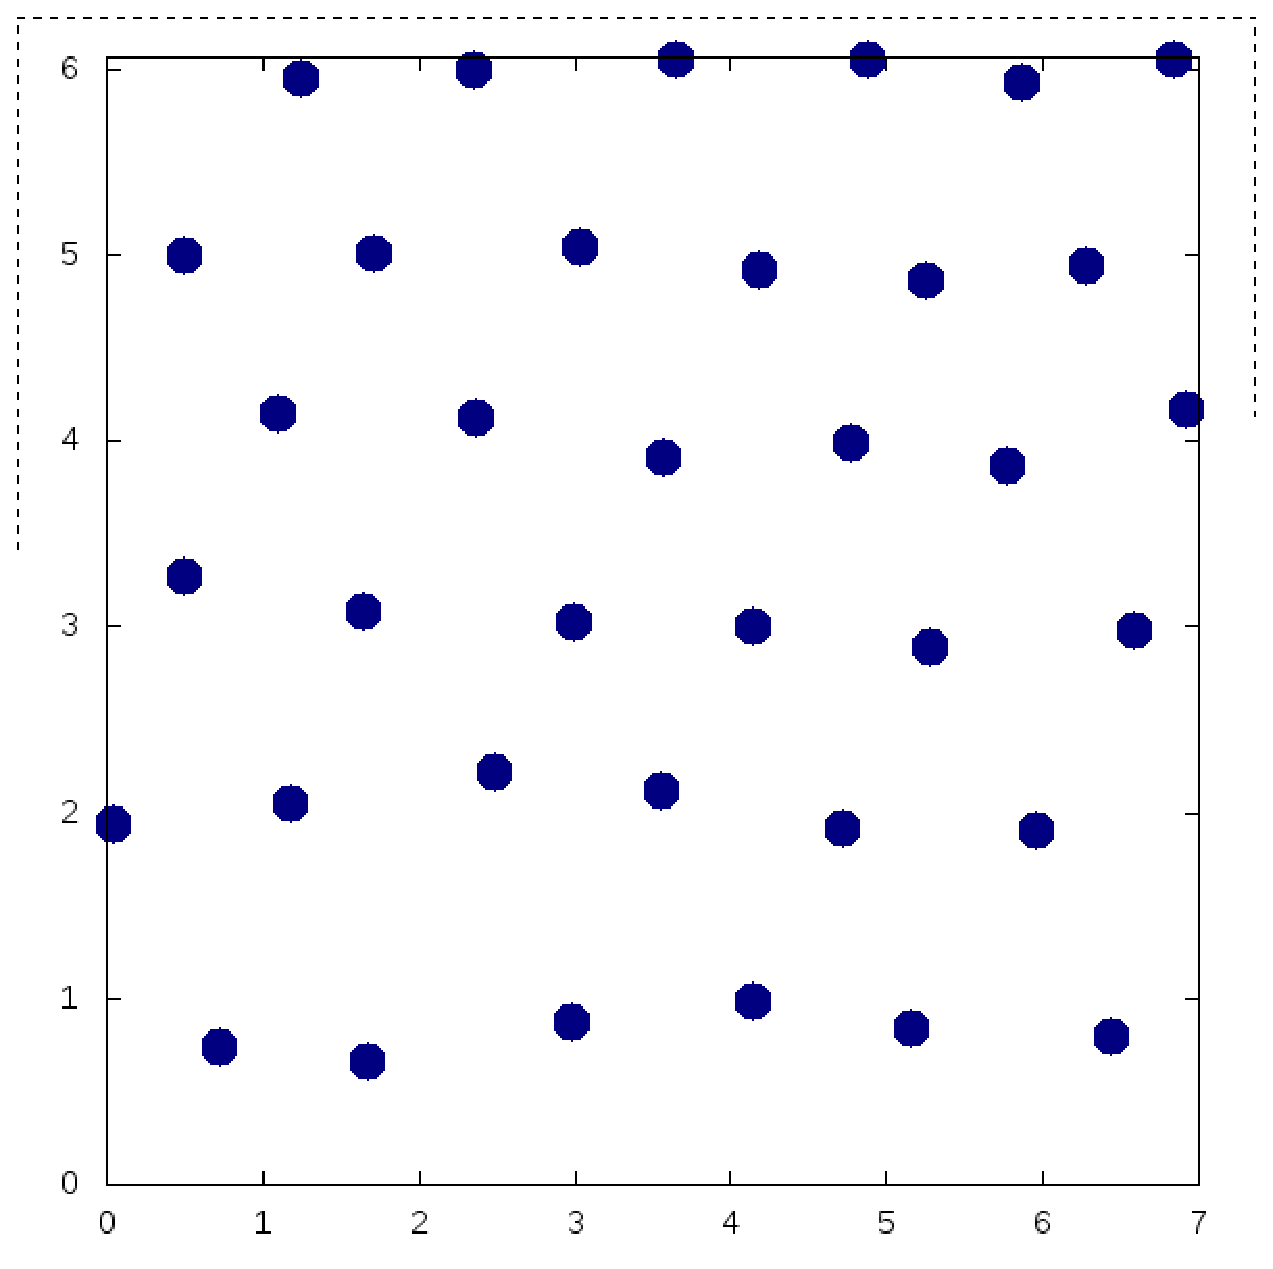
\includegraphics[width=0.6\linewidth]{pictures/system_crash}}
\caption{Состояние системы после некоторого числа шагов моделирования}
\label{ris:image13}
\end{figure}
  \begin{figure}[h!]
\center{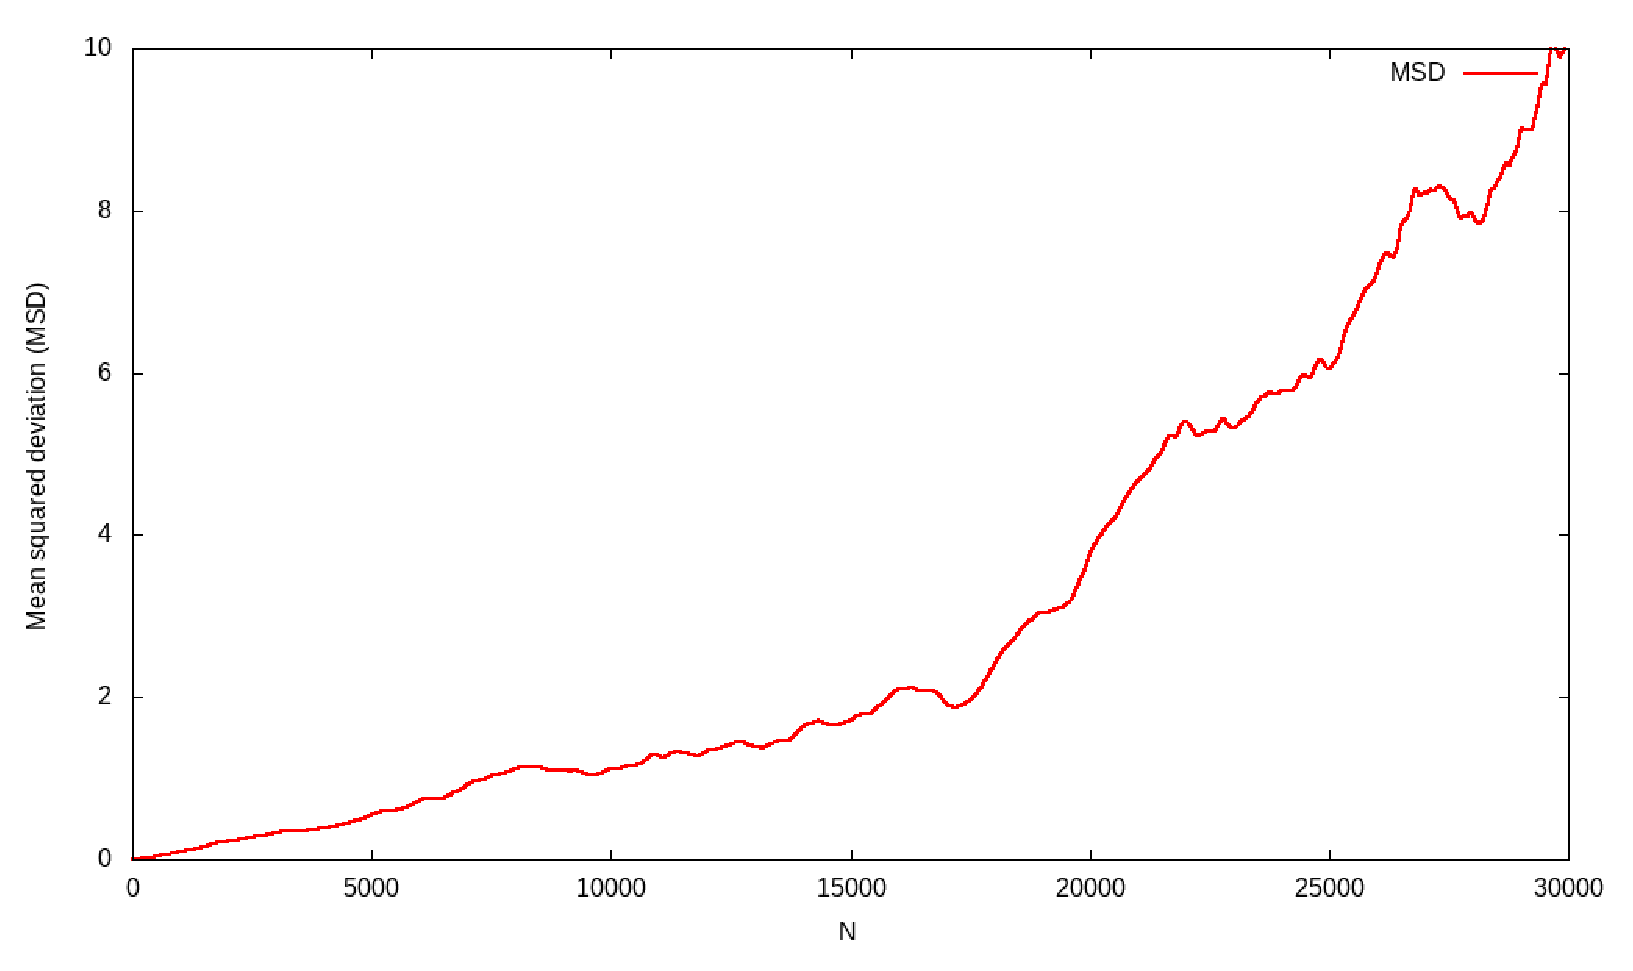
\includegraphics[width=0.6\linewidth]{pictures/MSD_crash_lie}}
\caption{График зависимости среднеквадратического смещения от номера шага алгоритма Метрополиса}
\label{ris:image14}
\end{figure}

В ходе решения поставленной задачи также не обошлось без вычисления дисперсии значений энергий системы в ходе моделирования.
Полученные значения данной величины следующие:
\begin{itemize}
\item $\sigma=0.00019255$ для квадратной решетки в устойчивом режиме;
\item $\sigma=0.00319038$ для квадратной решетки в неустойчивом режиме;
\item $\sigma=0,00000034$ для треугольной решетки в устойчивом режиме;
\item $\sigma=0.00447716$ для треугольной решетки в неустойчивом режиме;
\end{itemize}
Очевидно, что погрешности вычисления энергии для неустойчивых режимов обеих типов решетки выше. Причина этому заключается в том, что неустойчивый режим инициируется температурой системы, которая выше, чем в устойчивом режиме: вероятность частицы занять энергетически менее выгодное положение выше, чем в устойчивом режиме. 
\newpage\section{Выводы}
В ходе данной работы была разработана программа, моделирующая квазидинамику двумерной системы частиц, взаимодействующей через потенциал Леннарда-Джонса, с использованием алгоритма Метрополиса. Моделирование было проведено для квадратной и треугольной решеток с линейными размерами системы $L_x=7$  $L_y=\frac{\sqrt{3}}{2} L_x$ и квадратных решеток со стороной $L=L_x\sqrt{{\frac{\sqrt{3}}{2}}$, плотности которых равны при одинаковых параметрах $L_x$. Численный расчёт в ходе данной работы показал результаты, сходные с полученными в ходе выполнения прошлых работ, где использовался алгоритм Верле для моделирования динамики системы: система стремится принять положение с минимальной энергией, если температура системы достаточно мала.
\

После проведения расчётов были получены изображения,
показывающие расположение частиц в системах, а также были построены и проанализированы графики зависимости энергии систем в зависимости от шага моделирования. В ходе моделирования были задействованы параметры $\sigma$, полученные в ходе выполнения прошлой работы, при  которых энергия системы с квадратной или треугольной конфигурацией минимальна.
\

Из полученных в ходе исследования результатов можно сделать вывод, что треугольная структура решетки является более предпочтительной, поскольку обладает меньшей энергией при той же температуре. Вычисленные погрешности для четырех рассмотренных случаев показывают, что погрешность в вычислении энергии системы увеличивается с ростом температуры системы, поскольку вероятность принять конфигурацию с менее выгодной энергией выше.  Минимальна погрешность вычисления энергии у системы с начальной треугольной конфиругацией при низкой температуре, поскольку система изначально находится в энергетически выгодном состоянии из которого, в силу малости температуры, вероятность выйти мала относительно той же начальной конфигурации при большей температуре. 
\end{document}
